\documentclass{article}
 \usepackage[table,xcdraw]{xcolor}
%\documentclass[twocolumn,showpacs,showkeys,preprintnumbers,amsmath,amssymb]{revtex4}
\usepackage[american]{babel}
\usepackage[latin1]{inputenc}
\usepackage{graphicx}
\usepackage[colorinlistoftodos]{todonotes}
\usepackage{booktabs}
 \usepackage{booktabs}
\usepackage{float}
\usepackage{subcaption}
\usepackage{indentfirst}
\usepackage{natbib} 
\begin{document}


\title{Some title}

%\vspace{1cm}

\author{Marcelo V. Maciel \and Andr\'e C. R. Martins\\
	%}
	%\email{amartins@usp.br}
	%\affiliation{%
	NISC - EACH, Universidade de S\~ao Paulo\\
	Av. Arlindo B\'etio, 1000, S\~ao Paulo, 03828-080, Brazil}

%\author{Andr\'e C. R. Martins\\
	%}
 %\email{amartins@usp.br}
 %\affiliation{%
%NISC - EACH, Universidade de S\~ao Paulo\\
%Av. Arlindo B\'etio, 1000, S\~ao Paulo, 03828-080, Brazil}
 

\date{}


\maketitle
%\vspace{0.3cm}

%\center{\Large\bf Segundo autor}
%\center{\large\bf Afilia��o}


\begin{abstract}
	
	
	%\keywords{}
	%\pacs{}
\end{abstract}


\section{Introduction}

 % Incluir aqui a parte sobre teoria pol�tica, um par�grafo � suficiente, a princ�pio.

Here, we will present an opinion dynamics model
\cite{castellanoetal07,galam12a,galametal82,galammoscovici91,sznajd00,deffuantetal00,martins08a}
where the opinions exist over an one-dimensional axis and each agent has a best
estimate on more than one issue over that axis. Describing opinions over a
spatial landscape is an usual way to describe policy alternatives and agents'
preferences. The geometrical properties of the space are usually defined by
mapping from similarity and proximity of the political agents
\cite{downs1957economic, laver2014measuring}. Such a description can capture the
common notion of parties or policies being more ``to the left'' or ``right''. If
they're similar then they're closer \cite{van2005political, miller2015spatial}.
Major opinions, including political ones, tend to be formed not from only one
issue but from how each person feels about a number of them. Locating someone in
a left versus right or liberal versus conservative axis, therefore, requires
inspecting the opinions of that person in not only one but several issues that constitute the agent ideological positioning \cite{benoit2006party}.

For many problems, it makes sense to consider different issues as having components in
more than one single dimension \cite{vicenteetal08b}. However, it is often the case that describing the problem as
one-dimensional can be justified. We can certainly see this as a
first approximation along the most relevant dimension. In that case, the one dimensional case is
just a projection along a direction where variation seems especially important of higher-dimensional problems. From an application point of view, it is usual to find discussions to be simplified over only one main disagreement.  

One traditional way to model this type of scenario is to use continuous opinions
over a fixed interval, as it is done in the Bounded Confidence (BC) models
\cite{deffuantetal00,hegselmannkrause02}. While discrete models
\cite{galametal82,galammoscovici91,sznajd00} can be very useful at describing
choices, they are not easiest way to represent strength of opinion unless a
continuous variable is associated to the choice \cite{martins08a}. Discrete
models also tend to lack a scale where we can compare opinions and decide which
one is more conservative or more liberal.

On the other hand, continuous models are not particularly well suited for
problems involving discrete decisions. As we will not deal with those kinds of
problems here, they are a natural choice. Indeed, continuous opinions models
have been proposed for several different problems on how opinions spread on a
society \cite{deffuantetal02a,weisbuchetal05}, from questions about the spread
of extremism
\cite{amblarddeffuant04,gargiulomazzoni08a,franksetal08a,alizadeh14a,Albi2016,Mai2017}
to other issues such as how different networks
\cite{Kurmyshev2011,Acemoglu2011,Das2014,Hu2017} or the uncertainty of each
agent \cite{deffuant06} might change how agents influence each other.

Here, we will use a continuous opinion model created by Bayesian-like reasoning
\cite{martins08c}, inspired by the Continuous Opinions and Discrete Actions
(CODA) model \cite{martins08a,martins12b}. That model was shown previously
\cite{martins08c} to provide the same qualitative results as BC models. While a
little less simple, the Bayesian basis makes for a clearer interpretation of the
meaning of the variables. That makes extending the model and interpreting new
results simple. That approach is also consistent with a bounded rationality
variant interpretation of the spatial model of political decision making
\cite{humphreys2010spatial,ostrom1998behavioral}.

Variations of how each agent estimate how trustworthy other agents are will also
be introduced. Here, we use a function of trust $p^*$ that plays a role similar
to the threshold value in BC models. While $p^*$ is not a simple discontinuous
cut-off, it is a function of the distance between the opinions of the agent and
the neighbor. If only one issue is debated, that distance is uniquely defined.
However, if we have multiple issues represented on the same one-dimensional
line, it is not clear which distance we should use. That happens because we have
the opinion of agent $i$ on a specific issue $o_i$ and we can compare it to
$o_j$ to estimate how much $i$ trusts $j$. However, as there are several issues
we could also use the mean opinion of $i$ over all its issues and the same goes
for $j$. Therefore, we will study two additional cases: in the first
alternative, we will change \(p^*\) to \(p^{**}\), determined by the distance
between the neighbor and the agent average opinions. In the second alternative,
we will use a \(p^{***}\) calculated from the opinion of the neighbor and the
average opinion of the agent. The idea here is to make the behavior of our
agents closer to what experiments show about human reasoning. We have observed
that our reasoning about political problems can be better described as
ideologically motivated \cite{jostetal03a,taberlodge06a,Claassen2015a}. Indeed,
our opinions tend to come in blocks even when the issues are logically
independent \cite{jervis76a}. Our reasoning abilities seem to exist more to
defend our main point of views \cite{mercier11a,merciersperber11a} and our
cultural identity \cite{kahanetal11} than to find the best answer. In that
context, evaluating others by how they differ from us as a whole, instead of in
each issue, is a model variation worth exploring.
 
\section{The Model}


Here, the population will consist of  \(N\) agents fully connected (an agent $i$ can interact with any other agent $j$). Each agent $i$ will have an opinion $0\leq o_{i,k} \geq 1$, where $k=1, \ldots, n$ is a specific issue. We assume each agent opinion about issue $k$ can represented as a value $o_{i,k}$ at the range of possible values for $o$s. Agents also have an uncertainty $\sigma$ associated to their average estimate $o$. The uncertainty $\sigma$ could be different for each agent and also updated during the interactions \cite{martins08c}. For the sake of simplicity, however, we will assume the uncertainty $\sigma_i =\sigma$ is identical for (almost) all agents and it does not change. The set of opinions for each agent on all possible issues will define its ideological profile
\(I_i
=
(
(o_{i, 1}, \sigma),
\ldots,
(o_{i, n}, \sigma)
)
\)
, where \(n\) is the number of issues, \(o\) is
the opinion about the issue and \(\sigma\) is the global  uncertainty~\cite{martins12b}. The arithmetic mean  $x_i$  of agent $i$ opinions in each issue will be called here the ideal point for each agent, that is, it defines the agent ideological position at the
dimension of interest \cite{armstrong2014analyzing}. Obviously
\(
x_i
=
\frac{1}{n}
\sum_{k=1}^{n}
o_{k}
\).

In order to have agents with initial ideal points well distributed over the
possible range, the initial valued for each \(o_{i, k}\) was randomly drawn
using a Beta \(Be(\alpha, \beta)\) with random parameters $\alpha_i$ and
$\beta_i$. Those parameters were drawn for each agent $i$ from the ranges \( (
\alpha \in [1.1, 100], \beta \in [1.1, 100] ) \) by dividing those ranges by
\(N\) equally spaced values and then assigning them to each agent after mixing
the values. That is, if we have 10 agents one element of the following list of
possible pairs [(1.1, 56.0444), (23.0778, 34.0667), (45.0556, 100.0), (78.0222,
67.0333), (89.0111, 23.0778), (67.0333, 12.0889), (100.0, 78.0222), (56.0444,
1.1), (34.0667, 89.0111), (12.0889, 45.0556)] is assigned to each agent \(i\).
As a \(Be(\alpha, \beta)\) has an expected value of
$\frac{\alpha}{\alpha+\beta}$, that allows agents to start each simulation with
quite diverse value of ideal points. That also means the initial \(o_{i, k}\)s
of each agent $i$ will tend to be correlated.

For its part, \(\sigma\) is a parameter of the model, not the agents. However, a
proportion \textit{p$\_$intran} of the agents will have an unique \(\sigma_{i,k}
= 1e-20\). This is done so that we can control for the impact of inflexible
agents on the model dynamics \cite{galam05b,deffuant2002can,martinsgalam13a}.

How many agents are intransigent is also a parameter (coded as
\textit{p$\_$intran} ), and such \(\sigma\) is established at the initial
condition by sampling the issue index from the \(I_i\)'s length. This means that
we've opted for an implementation in which agents are intransigents in a
\textit{single} issue.

Each iteration of the simulation is the application of two procedures: the
opinion update through social influence and a random opinion update (noise). In
the social influence procedure we draw two agents, \(i\) and \(j\), from the
population, where \(i\) will observe \(j\) opinion about a specific issue \(k
\in (1 , \ldots, n)\). The issue $k$ is randomly drawn over its possible its
possible $n$ values. That way, we have the corresponding pairs (\(o_{i,k},
o_{j,k}\)) and (\(\sigma_{i,k}, \sigma_{j,k}\)). Finally, the agent \(i\)
updates its opinion (\(o_{i,k}\)) following a Bayesian rule: each agent has a
Normal prior \(f_i(\theta) = \frac{1}{\sqrt{2 \pi} \sigma_i} e^{- \frac{(\theta
    - o_i )^2}{2 \sigma_i}} \); for the likelihood there is an initial chance
\(p\), updated to \(p^*\) that the agent \(j\) has information and a chance
\(1-p\) it knows nothing and its opinion is just a random non-informative draw
which leads to \( f(o_j|\theta) = p N(\theta,\sigma_j^2) + (1-p)U(0,1) \); from
the expected value of the multiplication of the prior with the mixture
likelihood we derive the update rule \cite{martins12b}:

  \[
    o_{i,k}(t+1) =
    p^{*}
    \frac{o_{i,k}(t) + o_{j,k}(t) }{2}
    +
    (1 - p^{*})
    o_{i,k}(t).
  \]

  Wherein 
  \[
   p^{*}
    =
  \frac{
      p \frac{1}{\sqrt{2 \pi} \sigma_i}
      e^{- \frac{ (\Delta_{ij})^2}{2 \sigma_i^2}}
    }{
      p
      \frac{1}{\sqrt{2 \pi} \sigma_i}
    e^{- \frac{ ( \Delta_{ij})^2}{2 \sigma_i^2}}
    +
    (1 - p)
  }.
\]


%%%%%\todo[inline]{ Intransigents are intransigents over all issues or only one? This
%  is not clear in the text and the nomenclature $\sigma_{i,k}$ suggests it is
 % issue dependent. That must be explained. The update equations appear from
 % nowhere. They must be justified, no need to redo the calculations of the first
 % article. But we must say they come from a Bayesian update where each agent
 % assumes a Normal prior and a mixture likelihood. There is an initial chance p,
 % updated to p* the agent j has information and a chance 1-p it knows nothing
 % and its opinion is just a random non-informative draw. Include this! }

The \(\Delta_{ij} \) term is equal to \( o_{i,k} (t) - o_{j,k} (t)\). As
mentioned, we also test cases in which it's equal to \( x_i(t) - x_j(t) \) ( the
\(p^{**}\) case ) and to \(x_{i}(t) - o_{j,k}(t)\) ( the \(p^{***}\)). \(p\),
for its part, is a global parameter used to model the likelihood of the other
agent's (\(j\)) opinion being true \cite{martins12b}.

Furthermore, there is the noise: we draw another agent \(i\) whose opinion \(
o_{i,k}(t+1)\) is equal to \(o_{i,k}(t) + r\) where \(r\) is taken from a Normal
distribution of mean 0 and standard deviation \(\rho\). \(\rho\) is then a
global parameter of the simulation. From a theoretical point of view the noise
is justified as a way of accounting for the effect of factors not related to
social influence that make the agents change their opinion about issues
\cite{flache2017}. A further methodological justification is that small
perturbations in the local behavior of agents may lead to drastic changes in
systemic properties \cite{macy2015signal}. If an agent \(i\) is intransigent in
an issue \(k\) it won't randomly change its \(o_{i,k}\) opinion if its chosen by
the noise algorithm. Moreover, if \(o_{i,k}(t) + r > 1\) then \( o_{i,k}(t+1) =
1\). Likewise, if \(o_{i,k}(t) + r < 0 \) then \( o_{i,k}(t+1) = 0\).

  \section{Model Results}

  
  To have a general understanding about the model behavior we first established
  the bounds of the parameters:

% Please add the following required packages to your document preamble:
% \usepackage{booktabs}
% \usepackage[table,xcdraw]{xcolor}
% If you use beamer only pass "xcolor=table" option, i.e. \documentclass[xcolor=table]{beamer}
% Please add the following required packages to your document preamble:
% \usepackage{booktabs}
% \usepackage[table,xcdraw]{xcolor}
% If you use beamer only pass "xcolor=table" option, i.e. \documentclass[xcolor=table]{beamer}
  \begin{table}[H]
    \centering
\begin{tabular}{@{}|l|l|l|l|l|l|@{}}
\toprule
\rowcolor[HTML]{EFEFEF} 
$\sigma$ & $n$ & $p$ & $p\_intran$ & $N$ & $\rho$ \\ \midrule
$[0.01, 0.5]$ & $[1, 10]$  & $[0.1, 0.99]$ & $[0.0, 0.1]$ & $[500, 5000]$ & $(0.0, 0.1]$ \\ \bottomrule
\end{tabular}
\caption{Parameters' Bounds}
\end{table}

To sweep the parameter space we sample 70.000 parameterizations taken from
quasi-random low-discrepancy sequences \cite{saltelli2008global}, that generate
evenly spaced points. After running the simulation for 1.000.000 iterations we
take the  standard deviation of the population mean opinions (\(Ystd\)) as
a system final state measure. Histograms of the initial condition viz-a-viz
the three cases (\(p^{*}, p^{**}, p^{***}\)) final state lets us understand the
general tendency impinged by the update rules:

\begin{figure}[H]
  \centering
  
    \begin{subfigure}[b]{0.49\textwidth}
      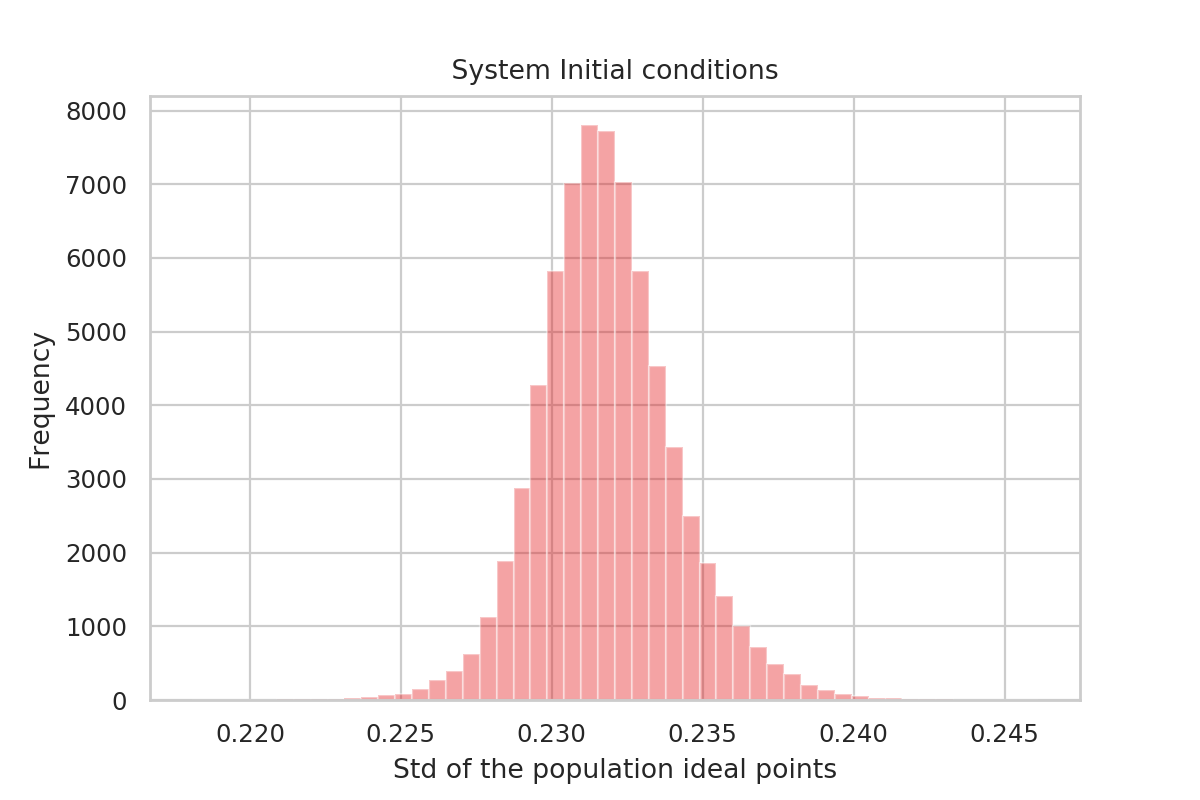
\includegraphics[width=\textwidth]{img/initstd.png}
%      \caption{\( n\_issues = 1,  \sigma = 0.1\) }
    \end{subfigure}
    \begin{subfigure}[b]{0.49\textwidth}
      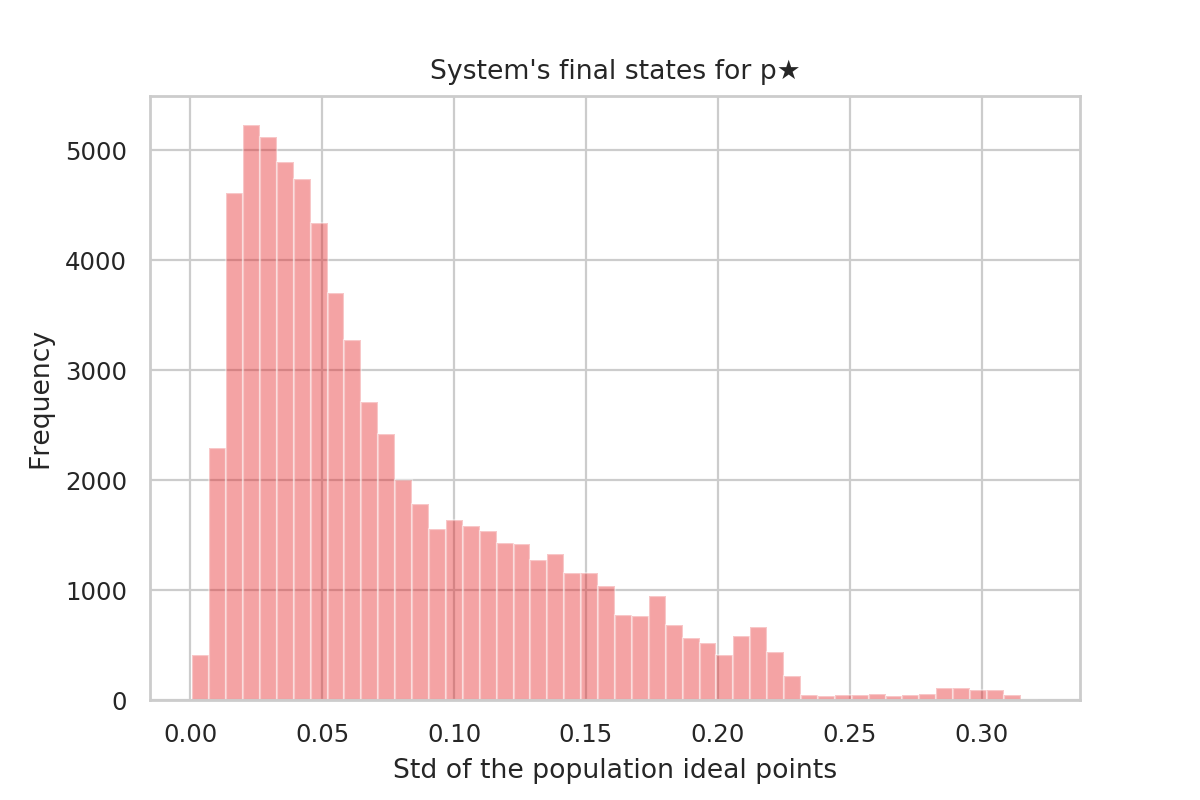
\includegraphics[width=\textwidth]{img/Ystd*.png}
 %      \caption{\(n\_issues = 1, \sigma = 0.02\) }
     \end{subfigure}

     \begin{subfigure}[b]{0.49\textwidth}
       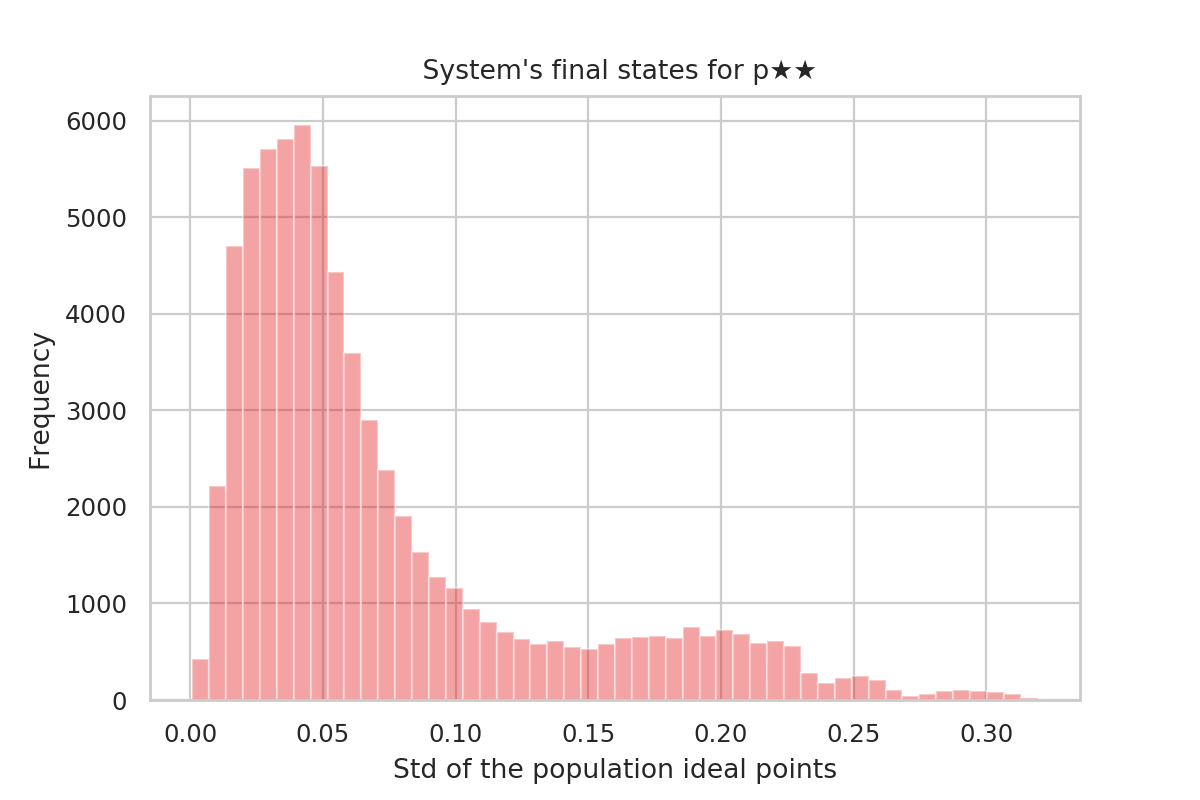
\includegraphics[width=\textwidth]{img/Ystd**.png}
  %     \caption{\(n\_issues = 7, \sigma = 0.1\)}
     \end{subfigure}
     \begin{subfigure}[b]{0.49\textwidth}
       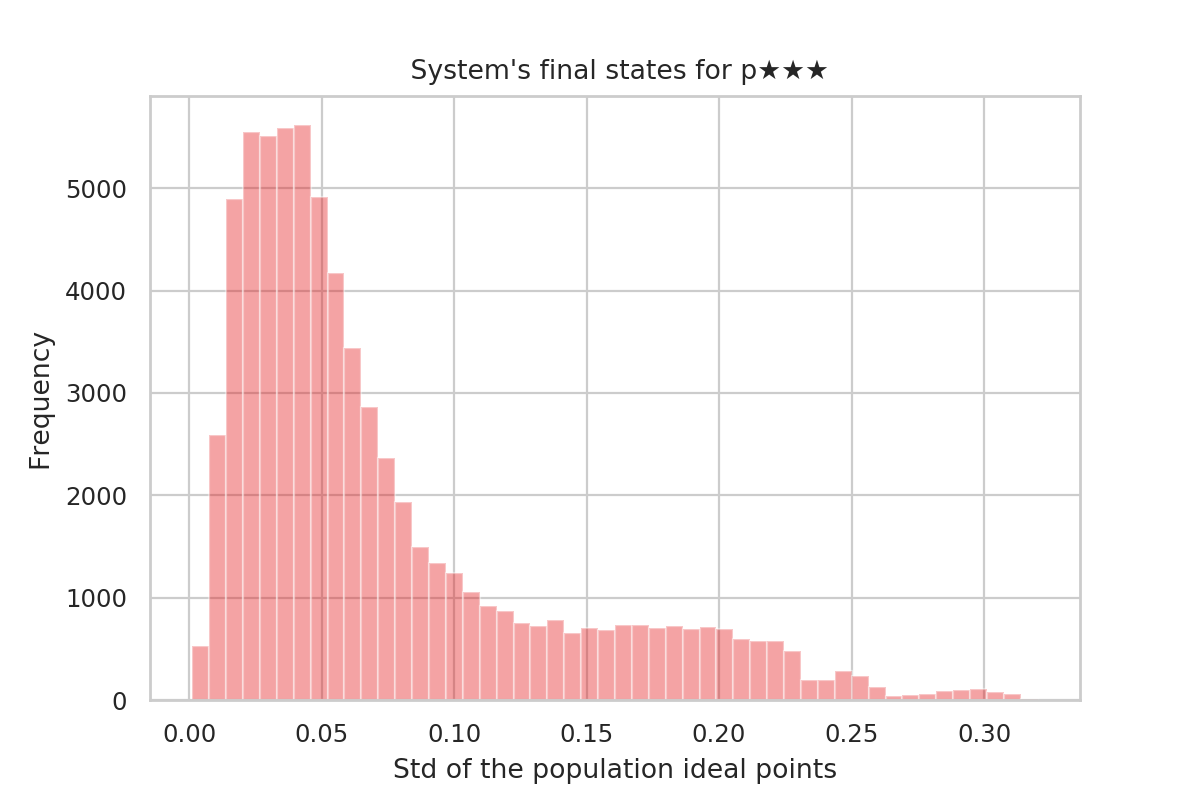
\includegraphics[width=\textwidth]{img/Ystd***.png}
   %    \caption{\(n\_issues = 7, \sigma = 0.02\)}
     \end{subfigure}
     \label{fig:hists}
     \caption{System initial condition x final state}
    \end{figure}

    The general tendency of the model is one of biased assimilation
    \cite{flache2017}. The histograms, however, don't show which parameter is
    the most important to explain this trend. With that in mind we perform a
    Sobol sensitivity analysis \cite{saltelli2000sensitivity} which generate the
    following indexes:

    \begin{figure}[H]
  \centering
  
    \begin{subfigure}[b]{0.45\textwidth}
      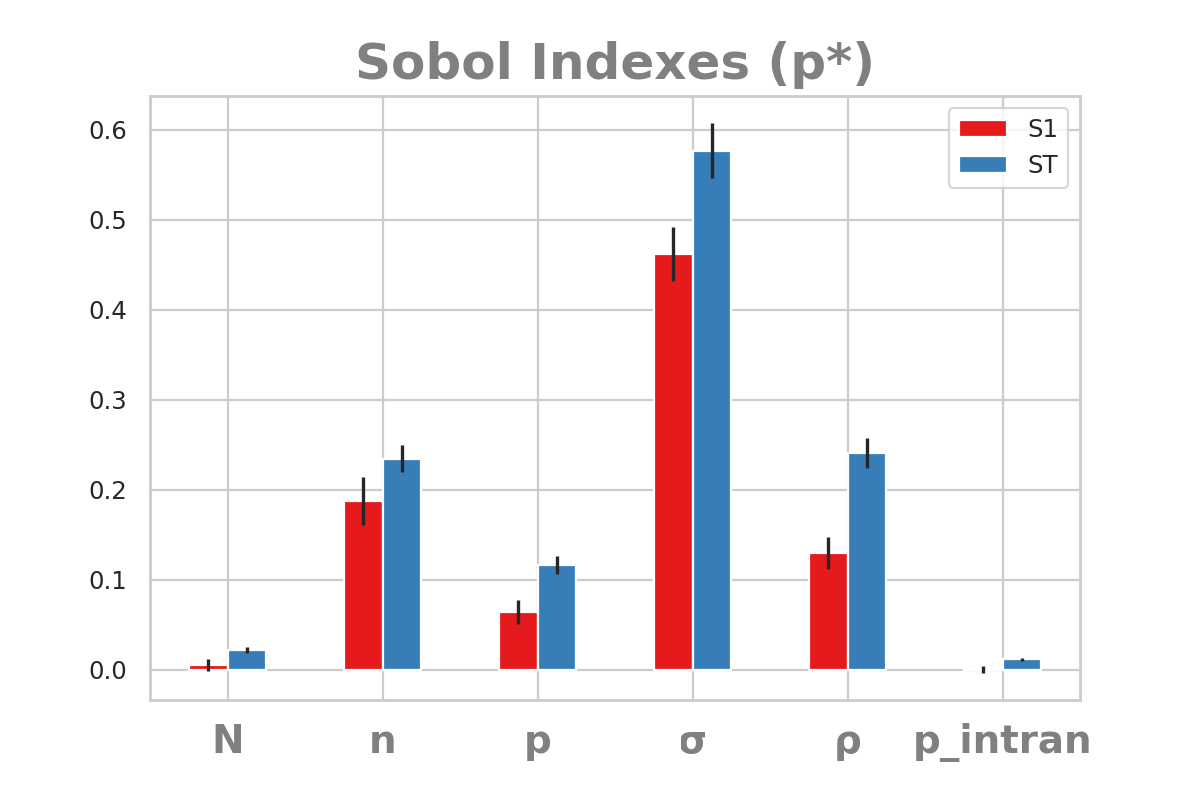
\includegraphics[width=\textwidth]{img/sobolpstar1.png}
%      \caption{\( n\_issues = 1,  \sigma = 0.1\) }
    \end{subfigure}
    \begin{subfigure}[b]{0.45\textwidth}
      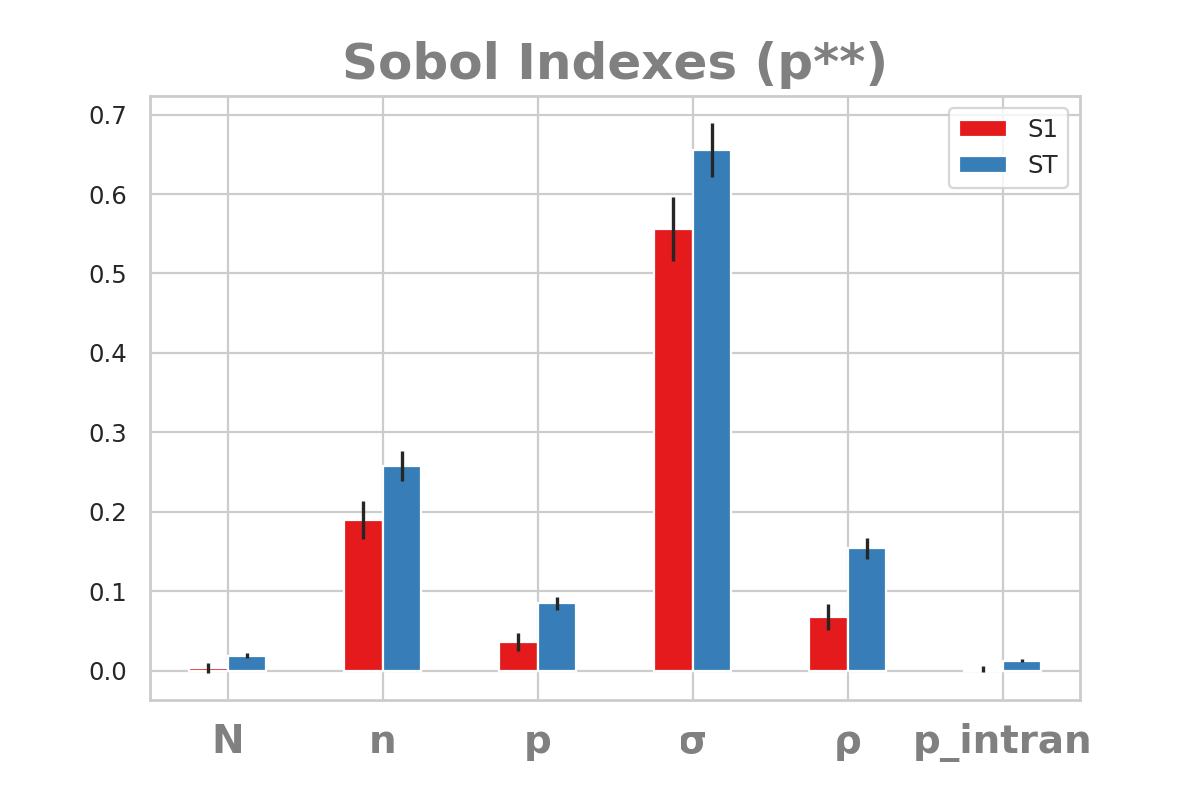
\includegraphics[width=\textwidth]{img/sobolpstar2.png}
 %      \caption{\(n\_issues = 1, \sigma = 0.02\) }
     \end{subfigure}
     \begin{subfigure}[b]{0.5\textwidth}
       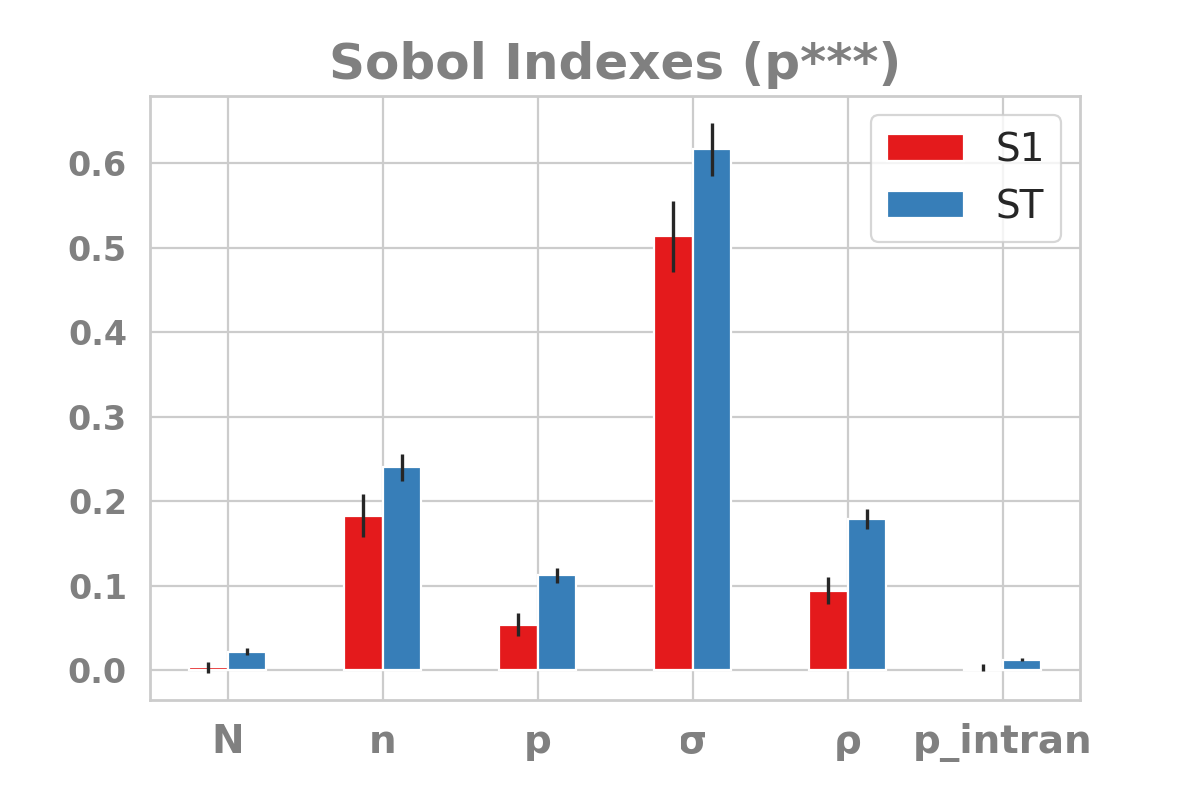
\includegraphics[width=\textwidth]{img/sobolpstar3.png}
  %     \caption{\(n\_issues = 7, \sigma = 0.1\)}
     \end{subfigure}
     \caption{Sobol Indexes for the three cases (\(p^{*}, p^{**}, p^{***}\))}
      \label{fig:sobolstuff}
    \end{figure}

    The sensitivity analysis shows that the most important parameters are :
    \(\sigma, n, \rho\), and that the three cases have the same qualitative
    behavior. \(\sigma\) being the parameter that explains the most the variance
    of the system measure is consistent with \citep{martins12b}, while the
    relevance of the number of issues and the noise is a new result. The
    sensitivity analysis, however, does not show the direction of the impact,
    which we investigate through scatter plots:

        \begin{figure}[H]
  \centering
  
    \begin{subfigure}[b]{0.45\textwidth}
      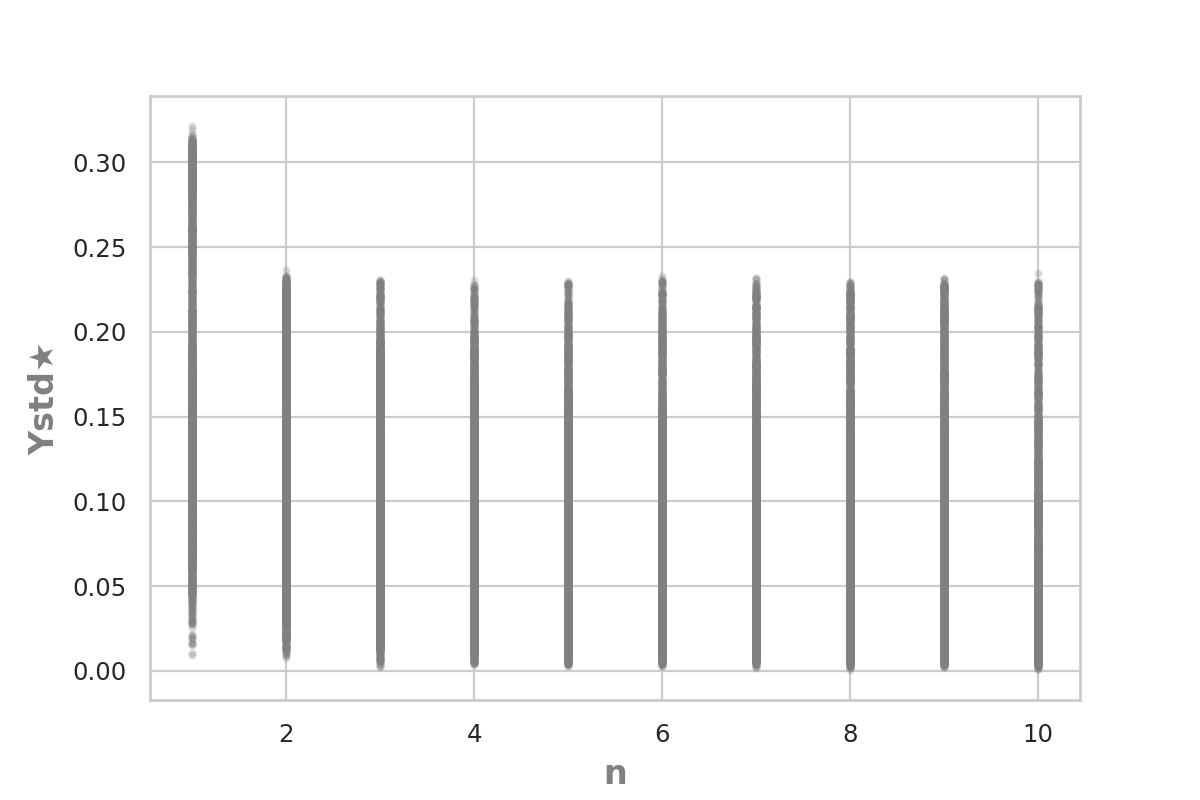
\includegraphics[width=\textwidth]{img/regressionYstd*n.png}
    \end{subfigure}
    \begin{subfigure}[b]{0.45\textwidth}
      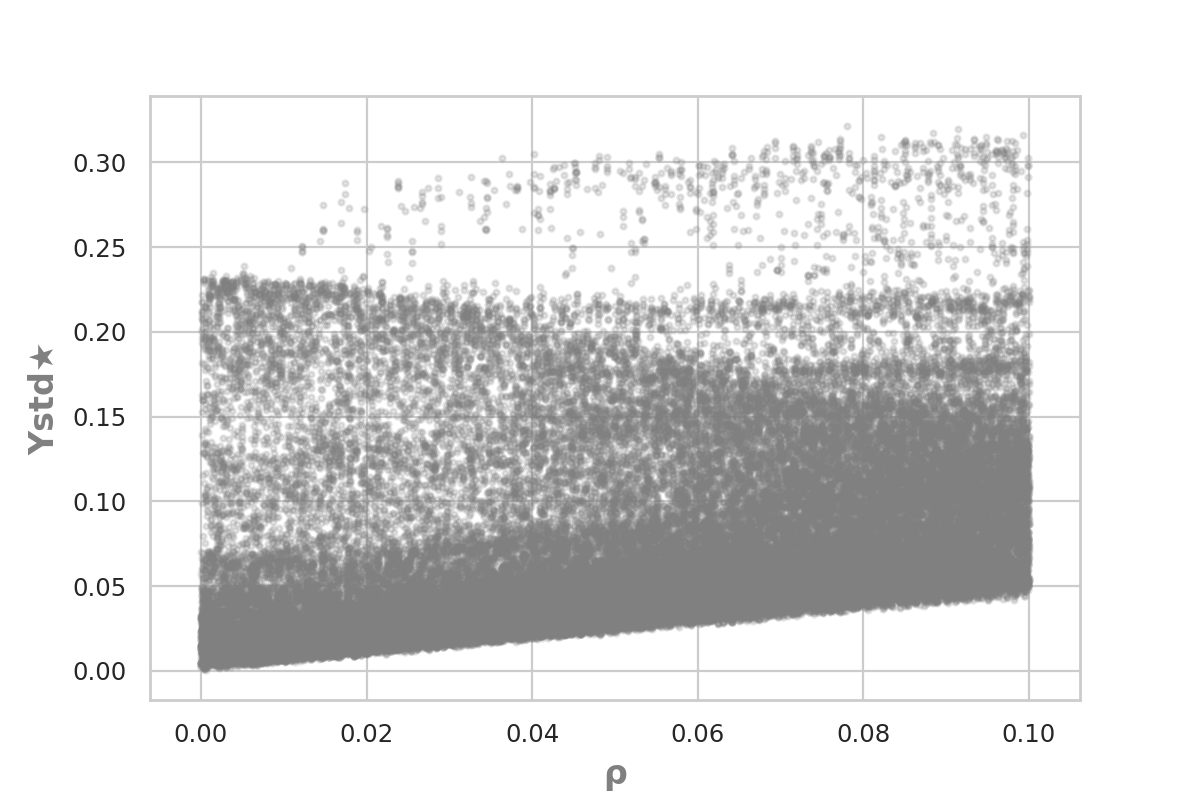
\includegraphics[width=\textwidth]{img/regressionYstd*rho.png}
 %      \caption{\(n\_issues = 1, \sigma = 0.02\) }
     \end{subfigure}
     \begin{subfigure}[b]{0.5\textwidth}
       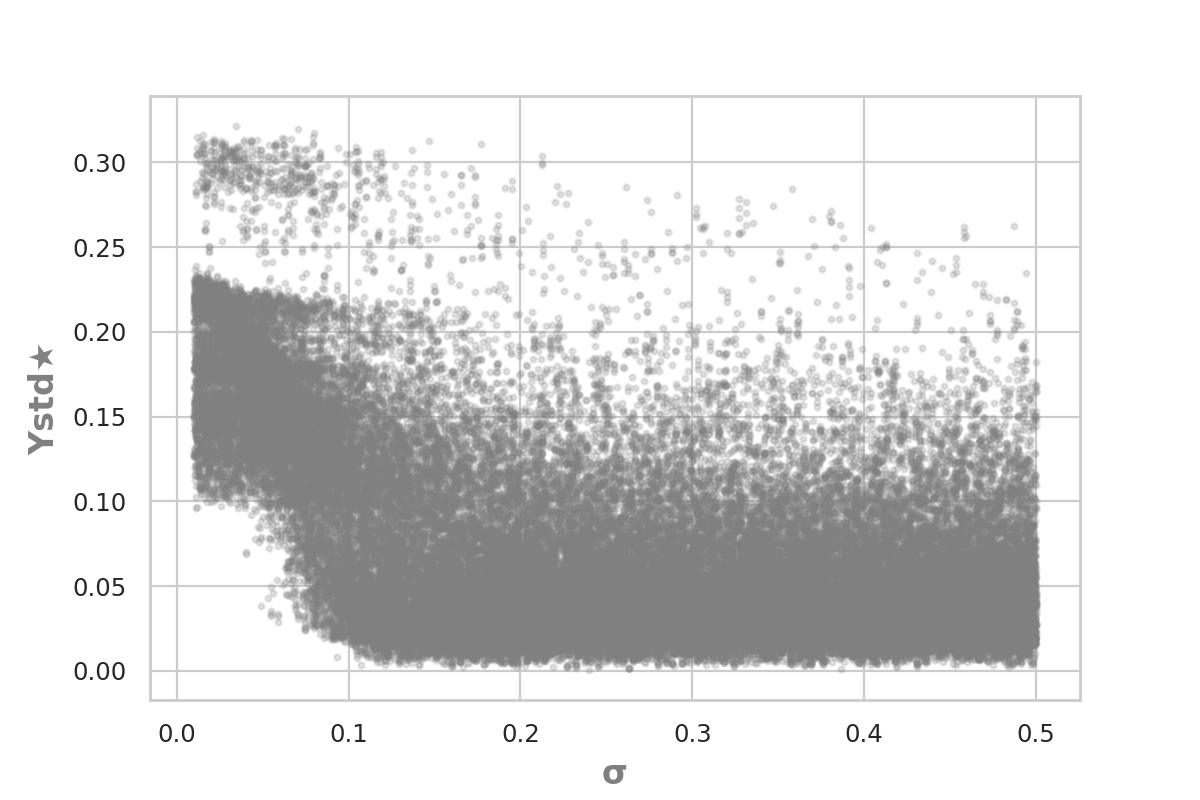
\includegraphics[width=\textwidth]{img/regressionYstd*sigma.png}
  %     \caption{\(n\_issues = 7, \sigma = 0.1\)}
     \end{subfigure}
     \caption{Scatterplots for the parameters with highest impact}
      \label{fig:scatters}
    \end{figure}

    The negative impact of \(\sigma\) in the population' opinion dispersion is
    to be expected given the update rule: a higher \(\sigma\) means that agents
    are easier to influence and as they're connected to all the others the more
    uncertain they the more centralized the agents' mean opinions after they
    interact with their neighbors. The plots also show that \(\sigma\) has the
    same impact on the system whenever its bigger than approximately
    0.1.Therefore we restrict our following analysis to the \((0.0, 0.1 ] \)
    range. The effect of \(\rho\) is also expected: the bigger the noise more
    dispersed is the final state of the system.

    After a general investigation we turn to the analysis of specific
    parametizations. For that let's start by fixing the following parameters as
    constants: \(\rho = 0.05 \) ; \(N = 500\) ; \(p\_intran = 0.0\), run the
    simulation for 500.000 iterations, and test combinations of $\sigma = (0.02,
    0.04, 0.1)$ and $ n = (1,5)$. As show by \ref{fig:tseries1}, \(\sigma\) has
    the effect of leading the dynamics of the simulation to the center as it
    increases: the bigger the \(\sigma\) the closest to the mean the population
    is . However,when the number of issues also increases that tendency is not
    clear, since the noise disperses them, even though \(\sigma\) has a bigger
    impact:


        \begin{figure}[H]
  \centering
    \begin{subfigure}[b]{0.45\textwidth}
      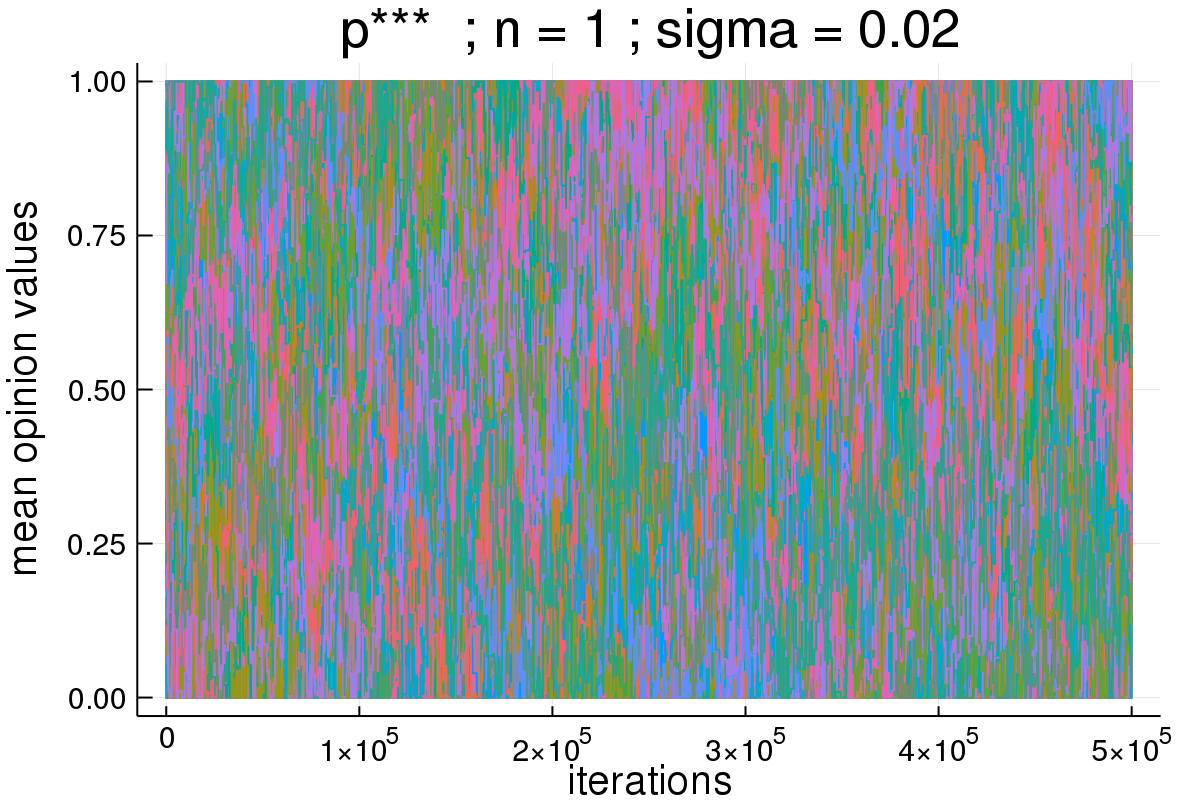
\includegraphics[width=\textwidth]{img/compare-ps/Poodlcalculatep***n1-rho005-sigma002-00intrans.png}
      %\caption{\textcolor{red}{'ill fix thix}}
    \end{subfigure}
    \begin{subfigure}[b]{0.45\textwidth}
      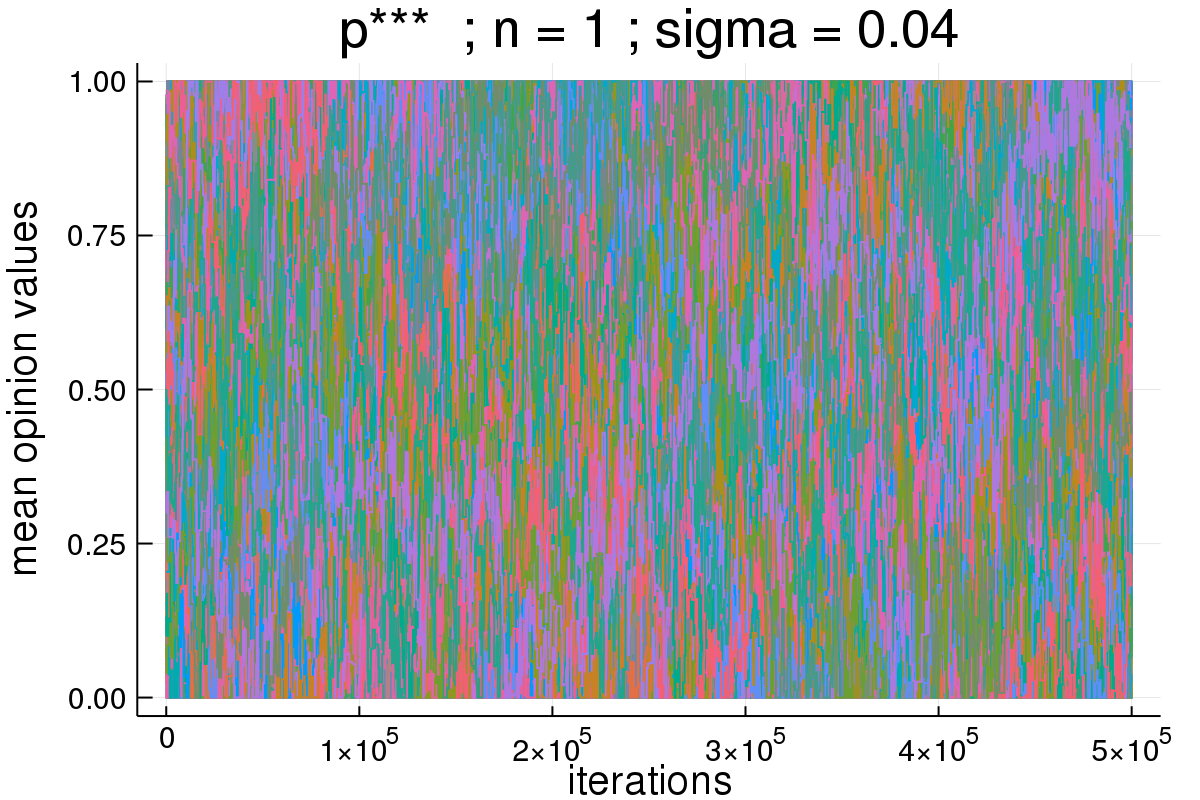
\includegraphics[width=\textwidth]{img/compare-ps/Poodlcalculatep***n1-rho005-sigma004-00intrans.png}
 %      \caption{\(n\_issues = 1, \sigma = 0.02\) }
     \end{subfigure}
     \begin{subfigure}[b]{0.5\textwidth}
       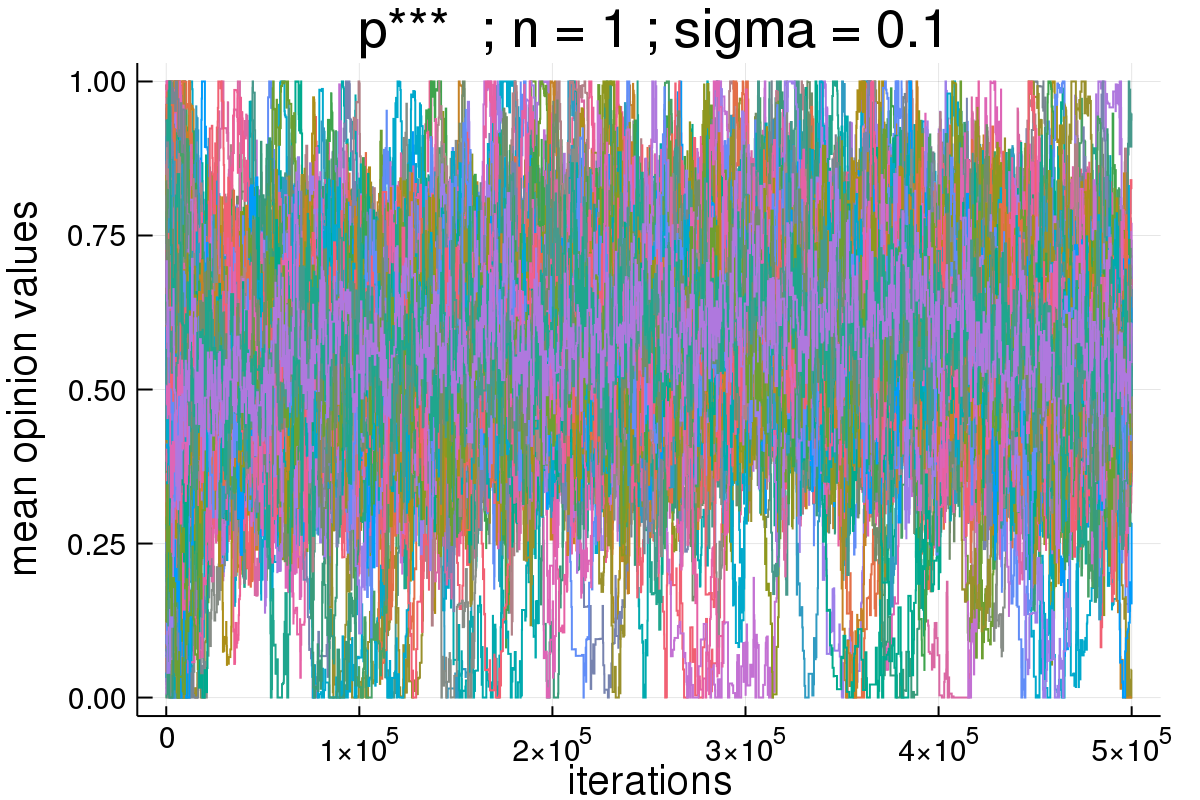
\includegraphics[width=\textwidth]{img/compare-ps/Poodlcalculatep***n1-rho005-sigma01-00intrans.png}
  %     \caption{\(n\_issues = 7, \sigma = 0.1\)}
     \end{subfigure}
     \caption{Time series for the parameterization: \(\rho = 0.05, N = 500,
       p\_intran = 0.0, n  = 1 \)}
      \label{fig:tseries1}
    \end{figure}

    On the other hand, when we also increase the number of issues the
    centralizing effect of \(\sigma \) becomes stronger:

    \begin{figure}[H]
      \centering
      \begin{subfigure}[b]{0.45\textwidth}
        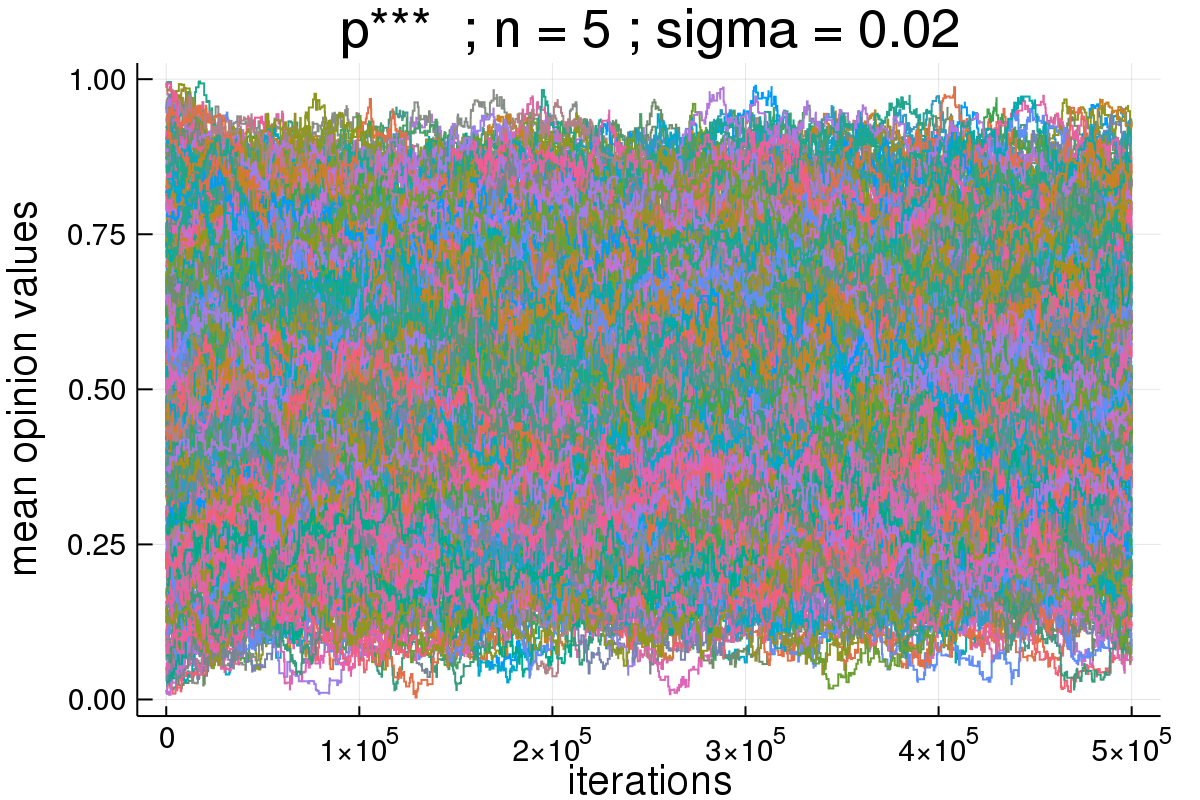
\includegraphics[width=\textwidth]{img/compare-ps/Poodlcalculatep***n5-rho005-sigma002-00intrans.png}
        % \caption{\textcolor{red}{'ill fix thix}}
      \end{subfigure}
      \begin{subfigure}[b]{0.45\textwidth}
        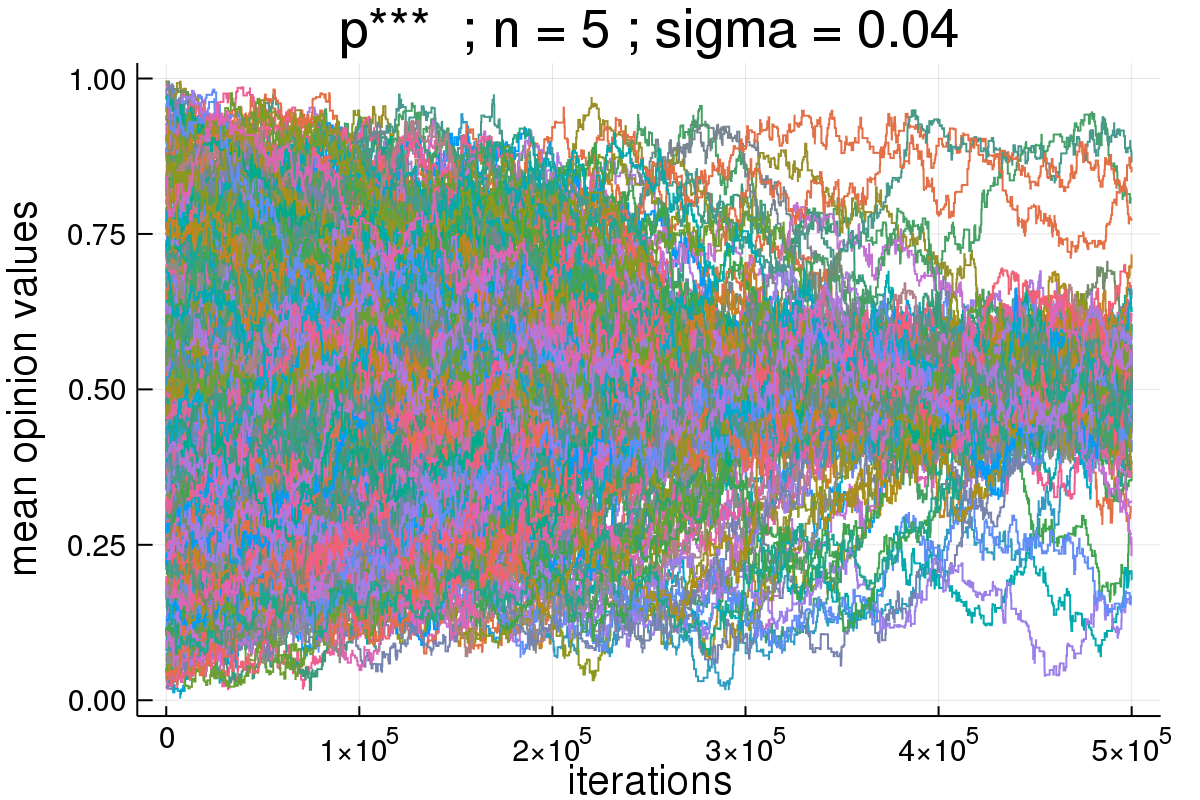
\includegraphics[width=\textwidth]{img/compare-ps/Poodlcalculatep***n5-rho005-sigma004-00intrans.png}
        % \caption{\(n\_issues = 1, \sigma = 0.02\) }
      \end{subfigure}
      \begin{subfigure}[b]{0.5\textwidth}
        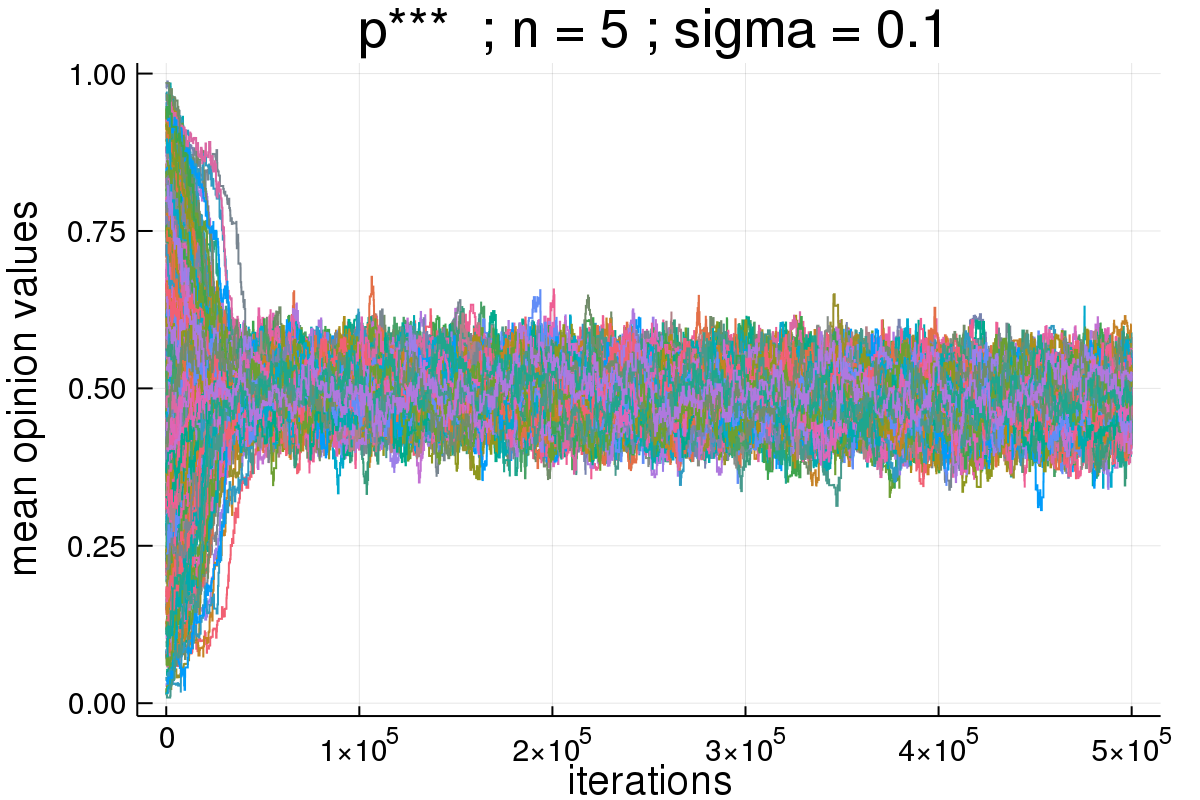
\includegraphics[width=\textwidth]{img/compare-ps/Poodlcalculatep***n5-rho005-sigma01-00intrans.png}
        % \caption{\(n\_issues = 7, \sigma = 0.1\)}
      \end{subfigure}
      \label{fig:tseries2}
      \caption{Time series for the parameterization: \(\rho = 0.05, N = 500,
       p\_intran = 0.0\)}
    \end{figure}

    The reason for that is : we're measuring the mean opinion values (\(x_i\))
    and \(\rho\) changes a single \(o_i\) at each iteration which means that a
    higher \(n\) implies a lesser impact of \(\rho\) on the mean opinion of the
    agent, since she will have \(n-1\) other opinions stabilizing her mean
    opinion at a point in the opinion spectrum. As \(\sigma\) is the parameter
    that dominates the model update rule it interacts with \(n\), which enforces
    \(\sigma\) effect whenever we test higher \(n\)s. This effect holds even
    when we raise \(\rho\) together with \(n\). Let's use the same
    parameterization as the last plot but with a new \(\rho\) such that \(\rho_2
    = \sqrt{n} * \rho_1 = \sqrt{10} * 0.05\). The interaction between \(n\) and
    \(\sigma\) still happens, with bigger \(n\) stabilizing the noise effect and
    contributing to the centralizing effect of \(\sigma\), even though a bigger
    \(\rho\) leads to more noise around the mean. 

    \begin{figure}[H]
      \centering
      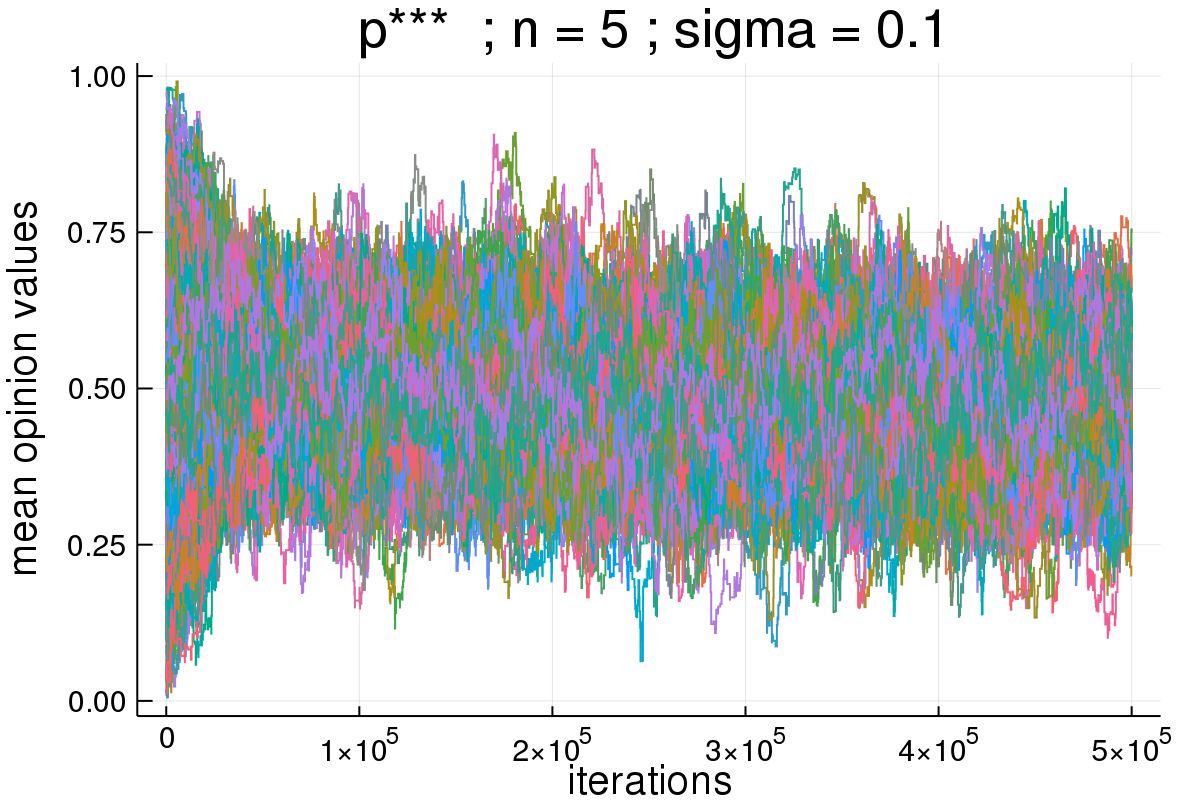
\includegraphics[width=0.9\textwidth]{img/compare-ps/Poodlcalculatep***n5-rho01118033988749895-sigma01-00intrans.png}
      \caption{Time series for the parameterization: \(\rho \approx 0.12, N =
        500, p\_intran = 0.0 \)}
      \label{fig:tseries3}
    \end{figure}

    Heretofore we've tested parameterizations with noise, but what happens if we
    lower \(\rho\) to a value close to zero, such as 1e-5? The first difference is
    that the population mean opinion values converge to certain values. In
    parameter combinations in which \(\sigma = 0.1\) the tendency is convergence
    to values close to 0.5. An interesting distinction between the cases in this
    parameterization is that \(p^{**}\) and \(p^{***}\) always converge to 0.5,
    independently of the number of issues. Alternatively, in the \(p^{*}\) case
    this happens when \(n=1\), but when we have \(n=5\) or \(10\) there are
    other values of convergence, more as we increase \(n\), even though the
    centralizing tendency remains.
    \begin{figure}[H]
      \centering
      \begin{subfigure}[b]{0.45\textwidth}
        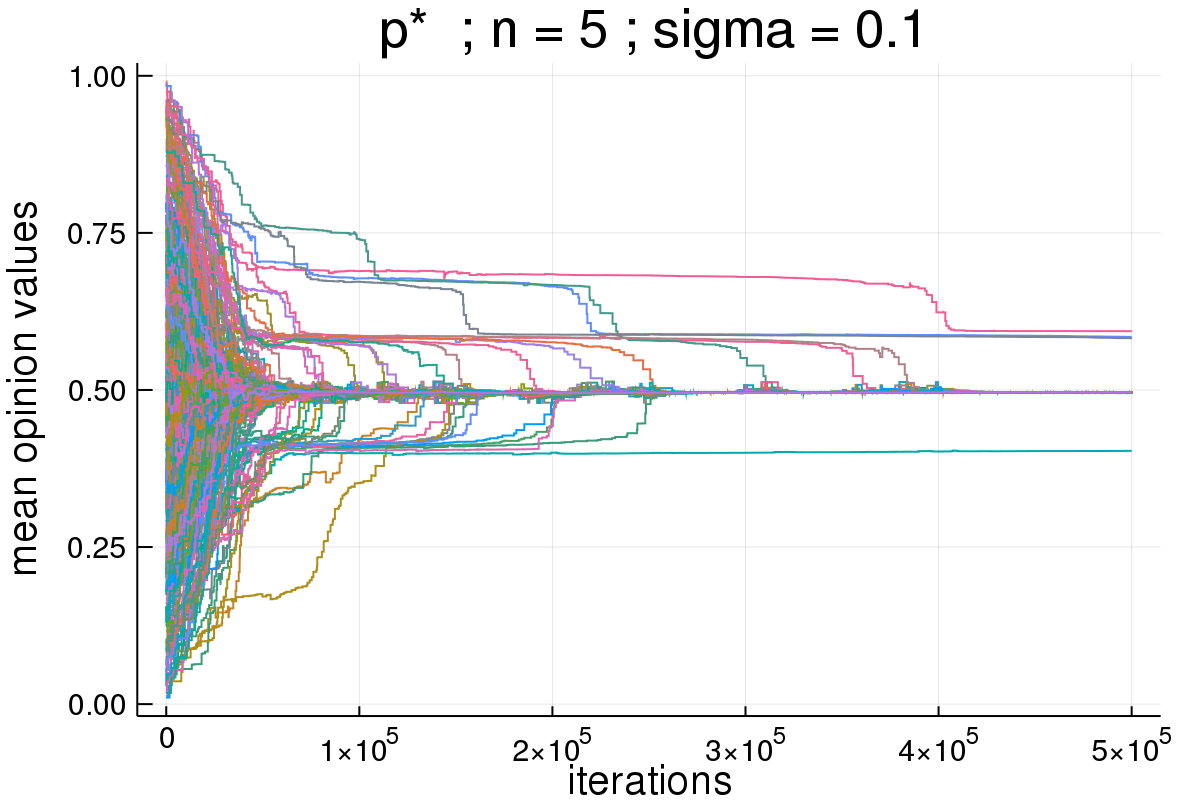
\includegraphics[width=\textwidth]{img/compare-ps/Poodlcalculatep*n5-rho10e-5-sigma01-00intrans.png}
        % \caption{\textcolor{red}{'ill fix thix}}
      \end{subfigure}
      \begin{subfigure}[b]{0.45\textwidth}
        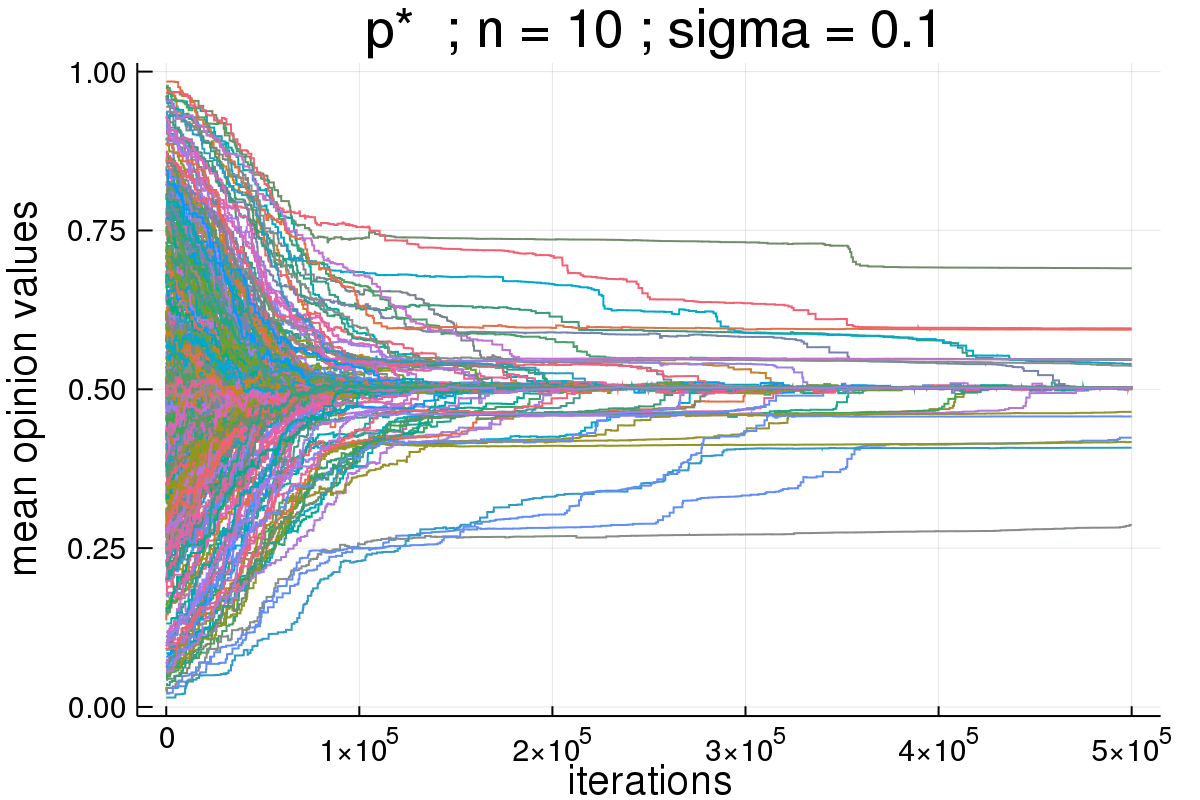
\includegraphics[width=\textwidth]{img/compare-ps/Poodlcalculatep*n10-rho10e-5-sigma01-00intrans.png}
        % \caption{\(n\_issues = 1, \sigma = 0.02\) }
      \end{subfigure}
      \begin{subfigure}[b]{0.5\textwidth}
        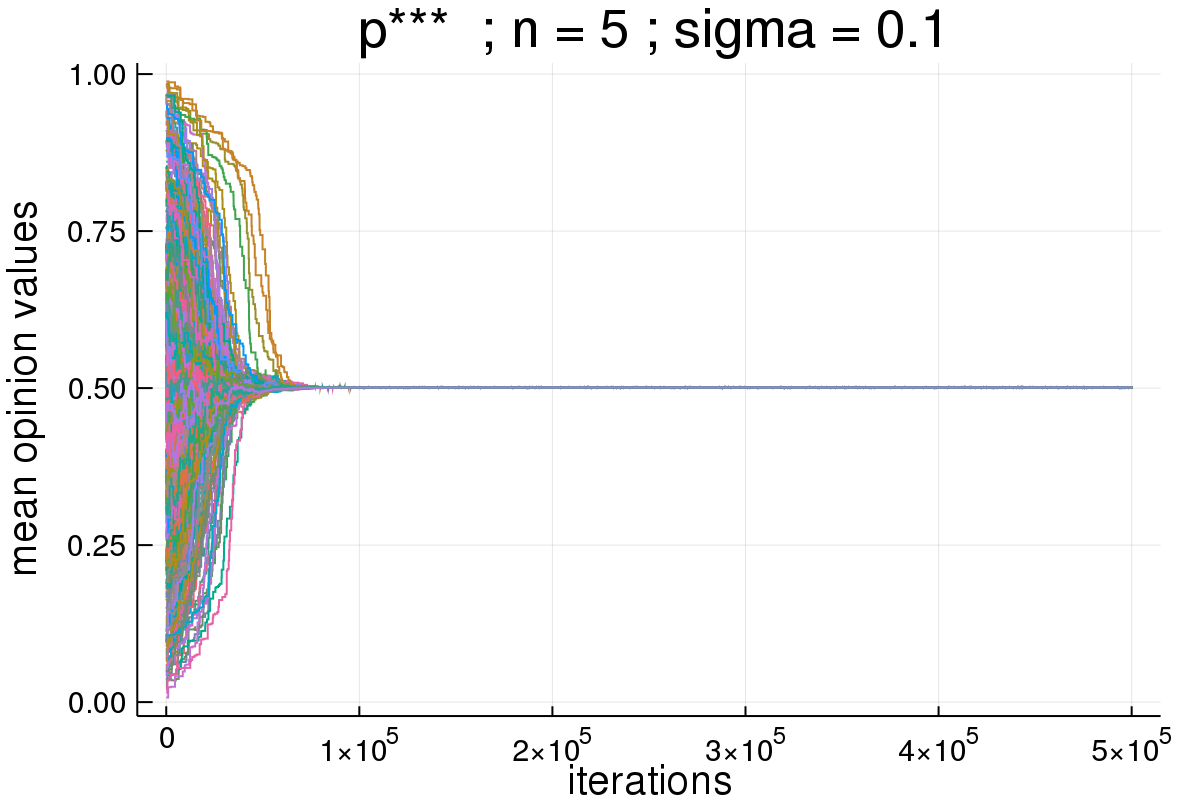
\includegraphics[width=\textwidth]{img/compare-ps/Poodlcalculatep***n5-rho1e-5-sigma01-00intrans.png}
        % \caption{\(n\_issues = 7, \sigma = 0.1\)}
      \end{subfigure}
      \caption{Time series for the parameterization: \(\rho = 1e-5, N =
        500, p\_intran = 0.0 \)}
      \label{fig:tseries4}
    \end{figure}
    In the parameterization in which \(\sigma\) is of intermediate value (for
    our range), such as \(0.02\) or \(0.04\), we observe another difference
    between cases: \(p^{*}\) has more convergence values than \(p^{**}\) and
    \(p^{***}\). Figure \ref{fig:tseries5} illustrates this system behavior:

    \begin{figure}[H]
      \centering
      \begin{subfigure}[b]{0.49\textwidth}
        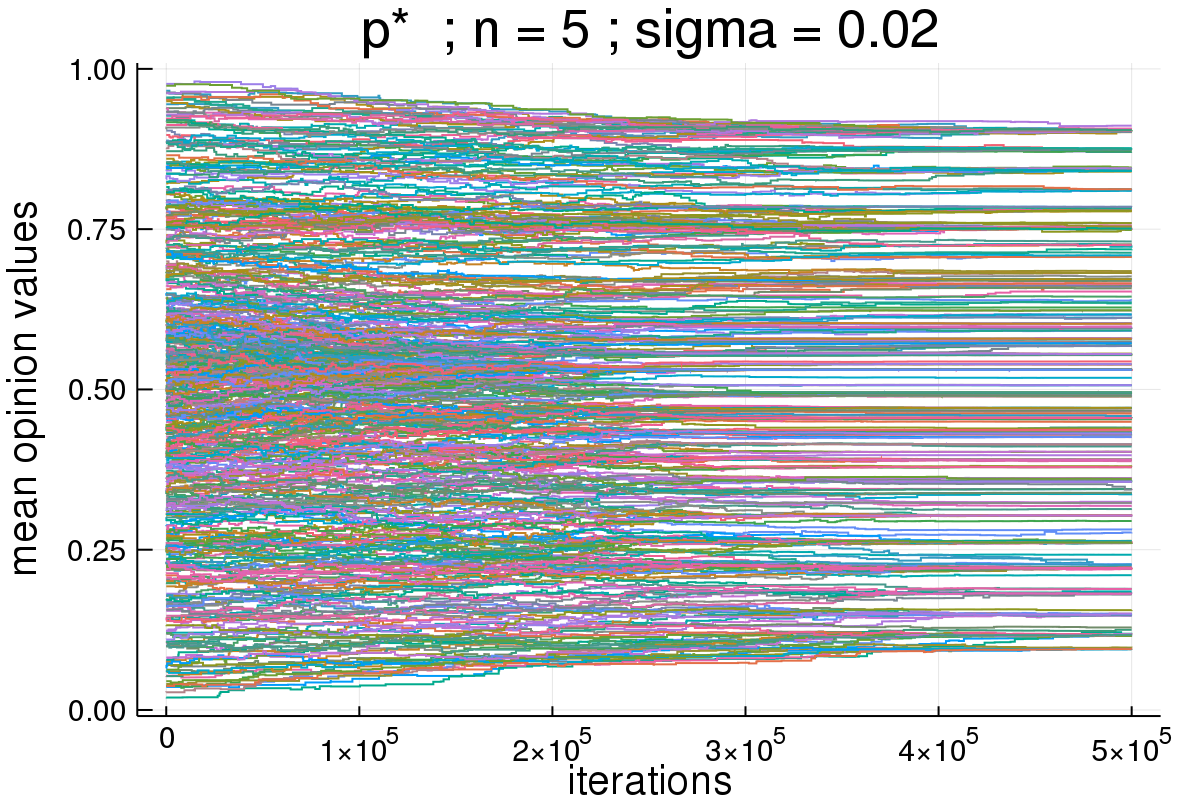
\includegraphics[width=\textwidth]{img/compare-ps/Poodlcalculatep*n5-rho10e-5-sigma002-00intrans.png}
        % \caption{\textcolor{red}{'ill fix thix}}
      \end{subfigure}
      \begin{subfigure}[b]{0.49\textwidth}
        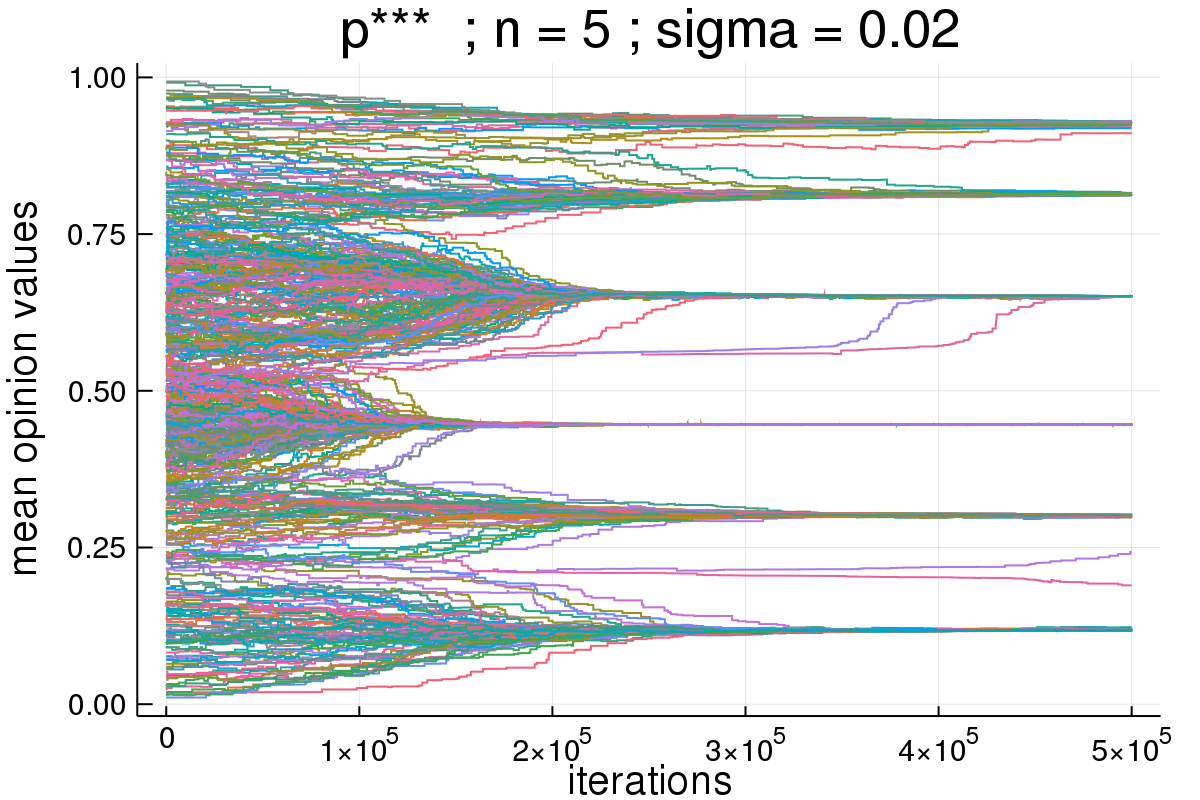
\includegraphics[width=\textwidth]{img/compare-ps/Poodlcalculatep***n5-rho10e-5-sigma002-00intrans.png}
        % \caption{\(n\_issues = 1, \sigma = 0.02\) }
      \end{subfigure}
      \caption{Time series for the parameterization: \(\rho = 1e-5, N =
        500, p\_intran = 0.0 \)}      
  \label{fig:tseries5}
    \end{figure}

    The reason for that lies in the \(\Delta\) of each case: in the \(p^{**}\)
    and \(p^{***}\) cases the update rules make use of mean opinion values which
    facilitates the opinion convergence. The \(p^{*}\) update rule works with
    single issue opinions which opens the possibility that there is little
    influence between agents given their ideological distance at the issue.
    
    Another impact of the number of issues, as shown in Figure
    \ref{fig:tseries6}, is that a higher \(n\) leads to a longer time for the
    convergence to certain values. The reason is that we're only changing one
    opinion by iteration, so naturally a higher \(n\) means the agents will take
    longer to be influenced. The relationship here is roughly linear such that
    the plot the region at \(5 \times 10^5\) iterations when \(n = 10\) is very
    similar to the corresponding region at \(0.5 \times 10^5\) when \(n = 1\).
    
    \begin{figure}[H]
      \centering
      
      \begin{subfigure}[b]{0.49\textwidth}
        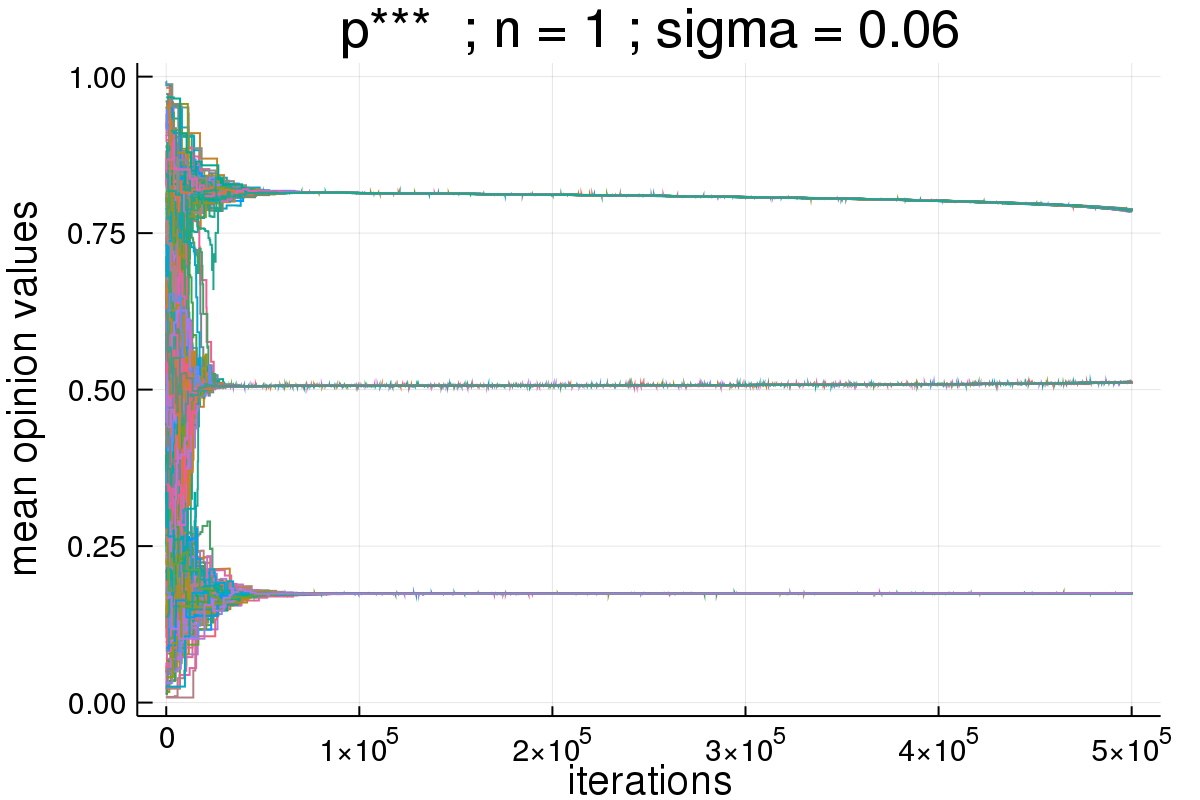
\includegraphics[width=\textwidth]{img/compare-ps/Poodlcalculatep***n1-rho10e-5-sigma006-00intrans.png}
        % \caption{\textcolor{red}{'ill fix thix}}
      \end{subfigure}
      \begin{subfigure}[b]{0.49\textwidth}
        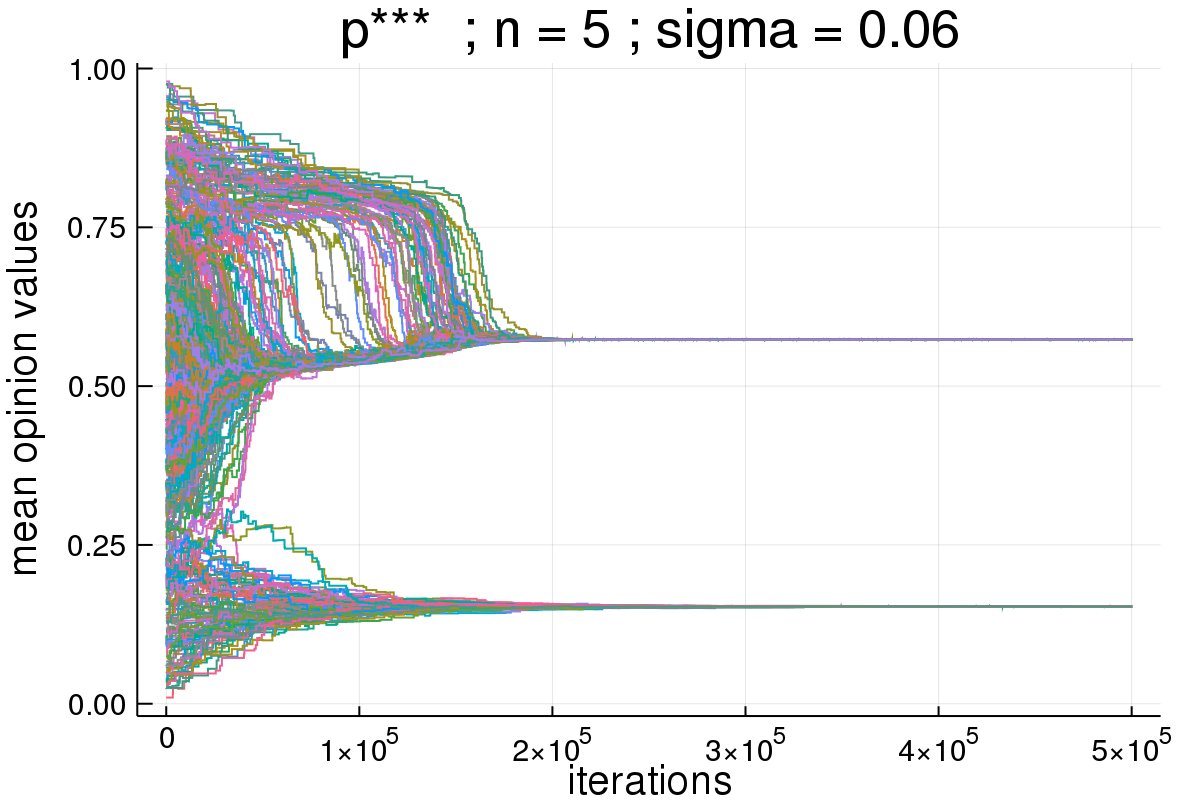
\includegraphics[width=\textwidth]{img/compare-ps/Poodlcalculatep***n5-rho10e-5-sigma006-00intrans.png}
        % \caption{\(n\_issues = 1, \sigma = 0.02\) }
      \end{subfigure}
            \begin{subfigure}[b]{0.49\textwidth}
        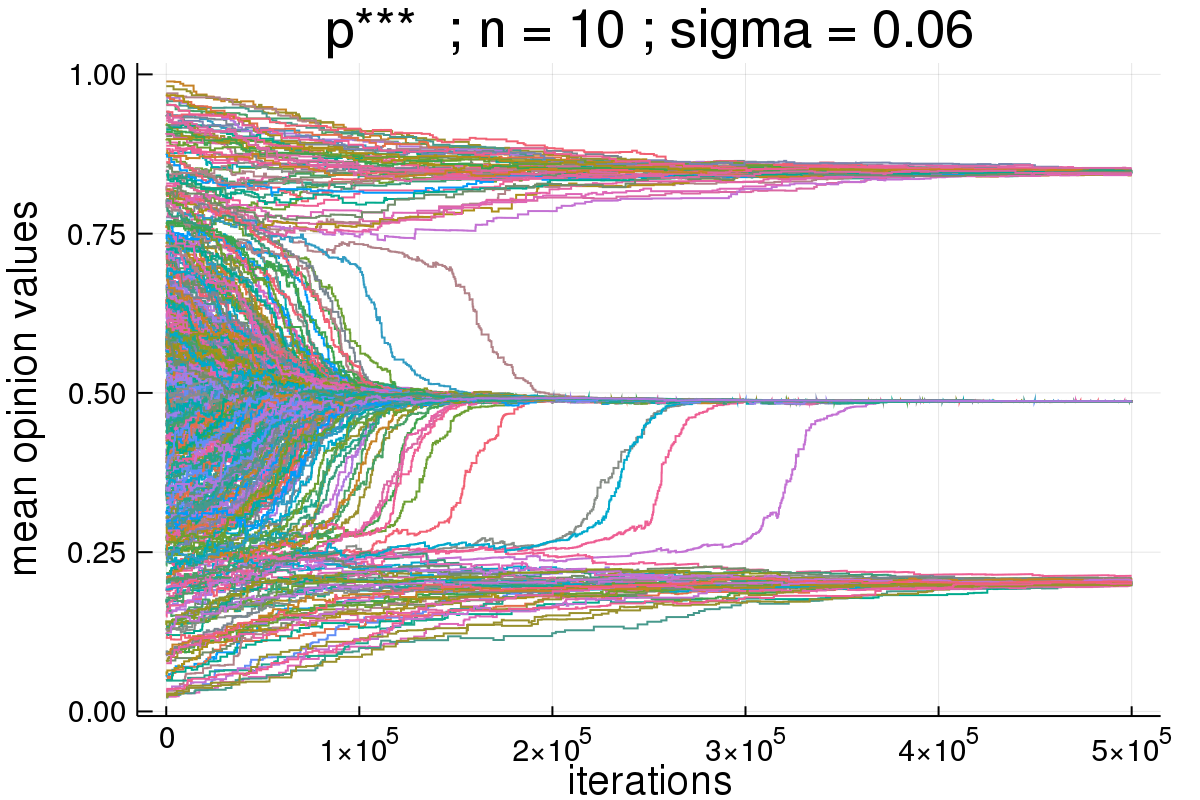
\includegraphics[width=\textwidth]{img/compare-ps/Poodlcalculatep***n10-rho10e-5-sigma006-00intrans.png}
        % \caption{\(n\_issues = 1, \sigma = 0.02\) }
      \end{subfigure}
      \caption{Time series for the parameterization: \(\rho = 1e-5, N = 500,
        p\_intran = 0.0 \).}
  \label{fig:tseries6}
    \end{figure}


    \todo[inline, color=yellow!30]{Should I talk about intransigents with
      \(\sigma = 0.01\) ???}
  \section{Conclusions}






\section{Acknowledgement}
The author would like to thank Funda\c{c}\~ao de Amparo \`a Pesquisa do Estado de S\~ao Paulo (FAPESP), for the support to this work, under grant %2008/00383-9.

\bibliographystyle{unsrt}
\bibliography{biblio}

\end{document}

%%% Local Variables:
%%% mode: latex
%%% TeX-master: t
%%% End:
